%%%%%%%%%%%%%%%%%%%%%%%%%%%%%%%%%%%%%%%%%%%%%%%%%%%%%%%%%%%%%%%
%
% Welcome to Overleaf --- just edit your LaTeX on the left,
% and we'll compile it for you on the right. If you open the
% 'Share' menu, you can invite other users to edit at the same
% time. See www.overleaf.com/learn for more info. Enjoy!
%
%%%%%%%%%%%%%%%%%%%%%%%%%%%%%%%%%%%%%%%%%%%%%%%%%%%%%%%%%%%%%%%
\documentclass[11pt]{article}
\usepackage[a4paper, margin=20mm]{geometry}
\usepackage{fontspec}
 
\setmainfont{Arial}

\usepackage{amsmath}
\usepackage{physics}

\usepackage{graphicx}
\graphicspath{ {./figs/} }
\usepackage{subfig}

%\renewcommand{\baselinestretch}{2}
\usepackage{setspace}
\doublespacing
\usepackage{titlesec}

\titlespacing\section{0pt}{0pt plus 0pt minus 0pt}{0pt plus 2pt minus 2pt}
\titlespacing\subsection{0pt}{0pt plus 4pt minus 2pt}{0pt plus 2pt minus 2pt}
\titlespacing\subsubsection{0pt}{0pt plus 4pt minus 2pt}{0pt plus 2pt minus 2pt}



\begin{document}
\section{Task 1: Lower Bound for Neural Network Output}
\label{sec:Task 1}
The method outlined in this task is essentially a trial-and-error approach to obtaining a lower bound to prove false properties. It is obvious that not all false properties are guaranteed to be proven false, especially for properties with mostly negative output domains. This means that even with very large values of \emph{k}, which would also be computationally expensive, there is always a chance that this method will miss a false property.
\subsection{Average amount of time taken to generate the outputs}
\label{sec:131}
 In order to avoid having to load the files 500\emph{k} times, we use an outer loop that loops through each file and an inner loop that loops through \emph{k}. We use the \emph{tic toc} function to get the time taken to generate the outputs for each $\emph{k}\in{\{1,2,3,....,K\}}$ for a single file, and store the values in a $(\emph{K}\times1)$ \emph{\textbf{individual\_time}} column vector. We then add up all the \emph{\textbf{individual\_time}} column vectors and divide by 500 element-wise to obtain the average amount of time taken to generate the outputs. When this data was plotted against \emph{k}, there were large spikes present in the plot. Given that the measured times were very short and \emph{tic toc} performs poorly when the code is too fast, the code was ran in a loop and the measured time was averaged for a single run \cite{tictoc}. The data is then plotted to give Figure \ref{fig:fig1a}. Not surprisingly, the average amount of time taken to generate the outputs tends to increase as \emph{k} gets larger. However, the large spikes are still present at the same positions of $\emph{k}=28,59,76$. This suggests that these spikes are not random events. One possible explanation is that these large spikes are intrinsic to the hardware of the device that the MATLAB code is being run on, due to the hardware-dependent behaviour of \emph{tic toc} \cite{hardware}.
 
\subsection{Average lower bound}
\label{sec:1.2}

We again use a nested loop with an outer loop that loops through each file and an inner loop that loops through \emph{k}. Each time the outputs are computed, we use the \emph{max()} function to determine the largest output, which would be the lower bound computed for that particular value of \emph{k}. In a similar way to what was done in Section \ref{sec:131}, a \emph{\textbf{lower\_bound}} row vector contains the lower bounds for each value of \emph{k} for a particular file. The row vectors are then added to one another and divided by 500 element-wise. The resulting row vector is then plotted against \emph{k}, giving Figure \ref{fig:fig1b}.



In Figure \ref{fig:fig1b}, the average lower bound increases significantly, before starting to level off at $\emph{k}=25$. The fact that the average lower bound is so low for small values of \emph{k} suggests that the output domains of most of the properties are largely, if not entirely, negative. This makes sense since 328 of the 500 properties are true, meaning that the output domains of a majority of the properties are entirely negative. As \emph{k} increases, the computed lower bound for each property starts to approach the upper limit of its respective output domain, which brings up the average lower bound. It should also be noted that the average lower bound remains negative even for very large values of \emph{k}, further confirming that most of the properties are true.

\subsection{Number of properties for which a counter-example was found}
\label{sec:1.3}

To obtain the number of counter-examples found for each value of \emph{k}, we again make use of the \emph{\textbf{lower\_bound}} row vector as well as a \emph{\textbf{false\_flag}} and a \emph{\textbf{total\_flag}} row vector (each initialised as a $1\times\emph{K}$ zero vector). A '1' is assigned to the \emph{k}\textsuperscript{th} element of \emph{\textbf{false\_flag}} if the \emph{k}\textsuperscript{th} element of \emph{\textbf{lower\_bound}} is positive. We do this for a single property and add \emph{\textbf{false\_flag}} to \emph{\textbf{total\_flag}}, before moving on to the next property and repeating the whole process. After looping through all 500 properties, \emph{\textbf{total\_flag}} can then be plotted against \emph{k} to obtain Figure \ref{fig:fig1c}. 



In Figure \ref{fig:fig1c}, it can be seen that the number of properties for which a counter-example is found generally increases as \emph{k} increases, which is expected. Since the \emph{k} inputs are randomly generated, a larger lower bound is more likely to be found if \emph{k} is large. The random generation of the \emph{k} inputs also explains the fluctuations in the plot. An increase in \emph{k} only increases the probability that a counter-example is found for a false property, it does not guarantee that a property for which a counter-example was found before will have a counter-example found again. In addition, it can also be observed that the plot starts to level off at around 50 to 60 proven false properties for larger values of \emph{k}. Since the total number of false properties is known to be 172, it is implied that it is relatively harder to find a counter-example for the remaining false properties, and that a far larger \emph{k} is needed to prove all the false properties are indeed false.

\begin{figure}[!htb]
  \centering
  \subfloat[Average amount of time taken to generate outputs (seconds) against \emph{k}]{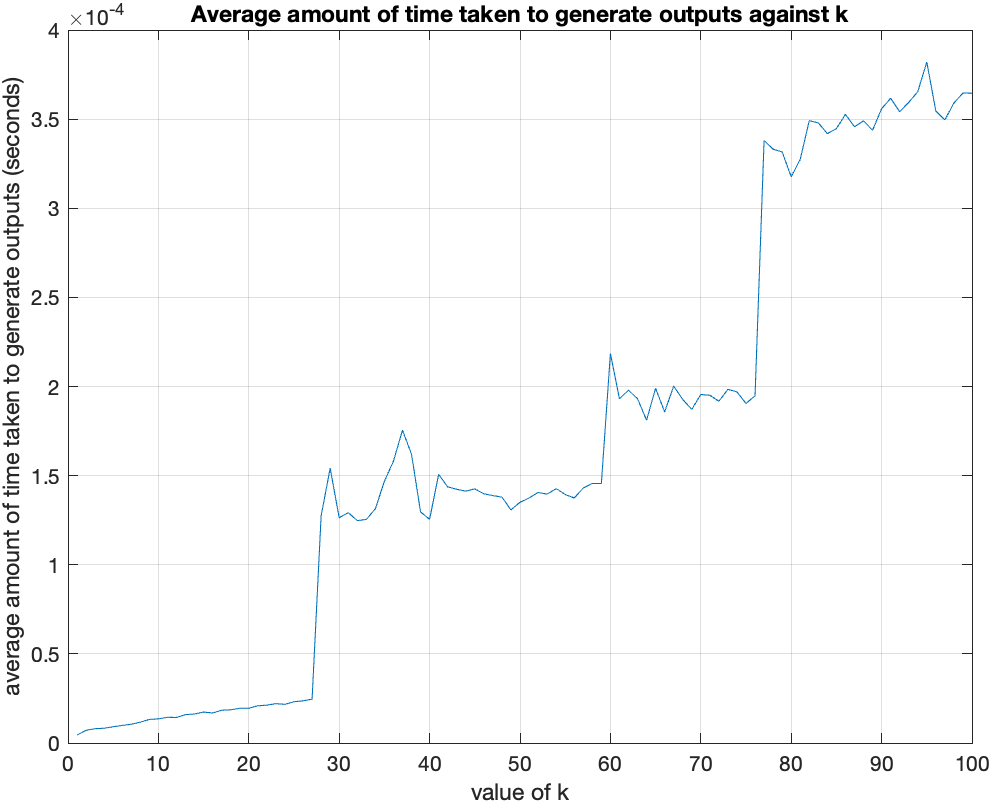
\includegraphics[width=5.6cm]{Task 1 (1000 times with grid).png}\label{fig:fig1a}}
    \hfill
  \subfloat[Average lower bound against \emph{k}]{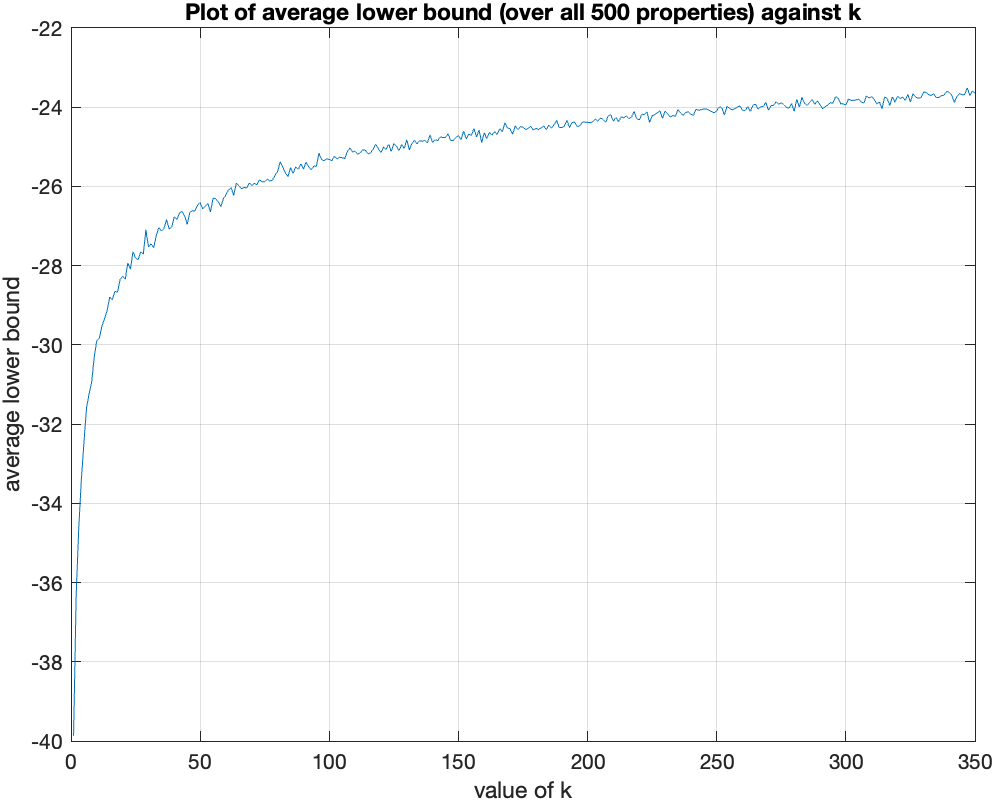
\includegraphics[width=5.6cm]{Task 1 average lower bound (over properties).png}\label{fig:fig1b}}
  \hfill
  \subfloat[Number of properties for which a counter-example was found against \emph{k}]{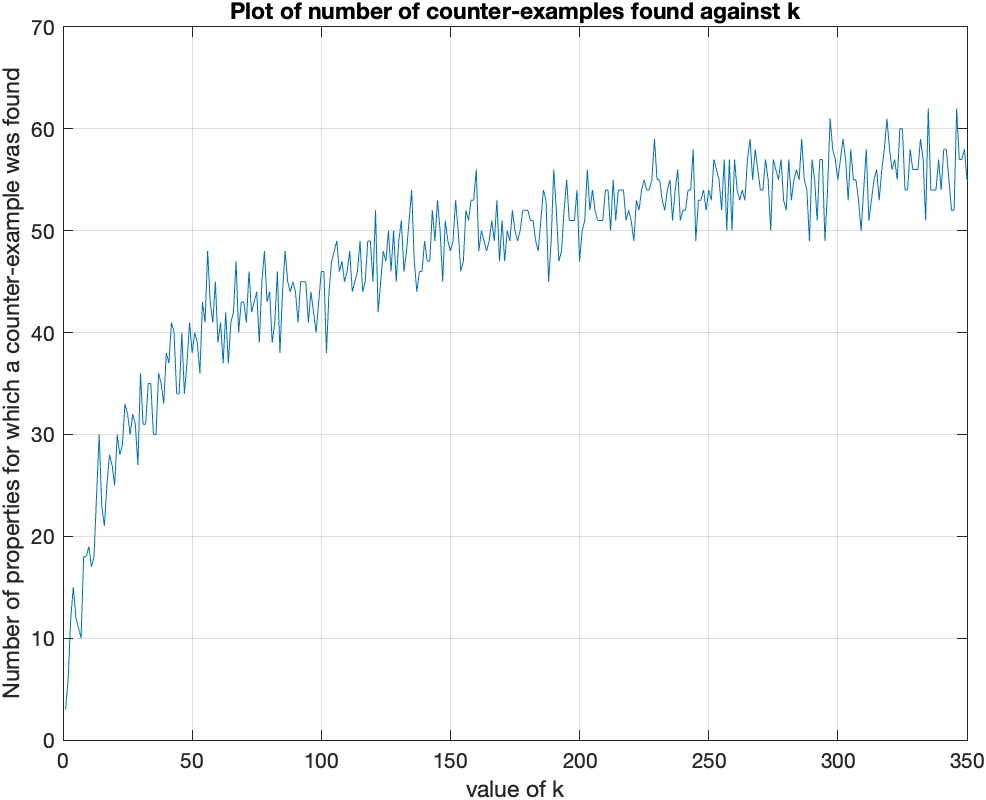
\includegraphics[width=5.6cm]{Task 1 counter example against k.png}\label{fig:fig1c}}
  \caption{Task 1}
\end{figure}


\section{Task 2: Interval Bound Propagation}
\label{sec:Task 2}

The modified weights $\ \textbf{W}_l^+$ and $\ \textbf{W}_l^-$ used in this method are modified in a rather simplistic way that loosens the bound constraints considerably. Hence, we do not expect this method to give very good lower and upper bounds. However, interval bound propagation is computationally inexpensive.

\subsection{Average values of the lower and upper bounds}
\label{sec:221}

The lower and upper bound for each property is computed using the \emph{interval\_bound\_propagation} function and cumulatively summed up in order to get the total lower bound and the total upper bound. Dividing both values by 500 would give an average lower bound of -137.882246646741 and an average upper bound of 82.7293950164992. From Figure \ref{fig:fig1b}, it can be seen that the average lower bound for $\emph{k}=350$ obtained in Task 1 is slightly larger than -24, which is far larger than the average lower bound computed using interval bound propagation. In fact, the average lower bound computed in Task 1 is larger than that computed in Task 2 even for small values of \emph{k}. Therefore, it seems that the method in Task 1 is superior to interval bound propagation at computing lower bounds.

%\lipsum[4] See Section \ref{sec:Task 2}.


\subsection{Number of properties proved}
\label{sec:222}

We initialise two $1\times500$ vectors (\emph{\textbf{false\_flag}} and \emph{\textbf{true\_flag}}) as zero vectors. \emph{if} statements are used to check the values of the lower and upper bounds of each property. If the lower bound of the \emph{i}\textsuperscript{th} property is positive, the property is false and a '1' is assigned to the \emph{i}\textsuperscript{th} element of \emph{\textbf{false\_flag}}. If the upper bound of the \emph{i}\textsuperscript{th} property is non-positive, the property is true and a '1' is assigned to the \emph{i}\textsuperscript{th} element of \emph{\textbf{true\_flag}}. The elements of \emph{\textbf{false\_flag}} and \emph{\textbf{true\_flag}} are then summed up separately at the end of the loop to give zero proven false properties and 11 proven true properties respectively. This confirms that interval bound propagation is inferior at proving false properties compared to the method in Task 1, which was able to prove some false properties even for small values of \emph{k}. Furthermore, interval bound propagation is only able to prove 11 out of the 328 true properties, which suggests that this method is not too good at proving true properties either. It can be concluded that interval bound propagation is unable to prove many properties because its computed bounds are too loose to be very useful.

\section{Task 3: Branch-and-Bound}
\label{sec:Task 3}

The branch-and-bound algorithm creates a rooted tree, which is a tree in which one vertex is set as the root \cite{Trees}, and evaluates all the leaf nodes (nodes with no children). In this case, the root is the original input domain ${\textbf{X}_{original}}$, and the leaf nodes are the subdomains. The branch-and-bound algorithm finds the leaf node with the highest upper bound and adds two children nodes to it (the subdomain with the largest upper bound is split into two new subdomains). Notice that this means smaller trees are contained within larger trees. This will be useful later.


\[
\emph{P} = \{{\textbf{X}_1},{\textbf{X}_2},{\textbf{X}_3},...,{\textbf{X}_n}\}, \qquad  \emph{\textbf{bounds}} = \begin{bmatrix}
{\Bar{y}_1}^{min} & {\Bar{y}_2}^{min} & {\Bar{y}_3}^{min} & ... & {\Bar{y}_n}^{min}
\\
{\Bar{y}_1}^{max} & {\Bar{y}_2}^{max} & {\Bar{y}_3}^{max} & ... & {\Bar{y}_n}^{max}\\
\end{bmatrix}^T
\]

As shown above, we use a cell array \emph{P} in the code to contain the set of the subdomains obtained so far. We also use a matrix \textbf{\emph{bounds}} to store the lower and upper bounds. ${{\Bar{y}_j}^{min}}$ and ${{\Bar{y}_j}^{max}}$ are the lower and upper bounds respectively for the neural network output computed when the input is restricted to ${\textbf{X}_j}$, where $\emph{j}\in{\{1,2,3,...,n\}}$. Since we know the method in Task 1 is superior at computing the lower bound, interval bound propagation is only used to compute the upper bound while the Task 1 method (using 20 inputs in this case since the average lower bound in Task 1 starts levelling off at around $k=20$) is used to compute the lower bound.


After the subdomain ${\textbf{X}_J}=[{\textbf{x}_J}^{min},{\textbf{x}_J}^{max}]$ with the largest upper bound is found, ${\textbf{X}_J}$ is split into two new subdomains. The lower and upper bounds for the two new subdomains are computed using the Task 1 method and interval bound propagation respectively. The two new subdomains are added to \emph{P} while ${\textbf{X}_J}$ is removed. The respective bounds are also added to and removed from \textbf{bounds}. Of course, the lower and upper bounds are checked between partitions, and the algorithm is terminated if the property is proven.

\subsection{Execute}

We want to perform \emph{p} partitions, and obtain the number of verified properties as well as time taken for the branch-and-bound algorithm, and plot the former against the latter. Hence, it is tempting to use a nested loop to loop through each property for each value of \emph{p} in order to find the time taken and the number of proven properties for each value of \emph{p}. However, as mentioned before, smaller trees (less partitions) are contained within larger trees (more partitions). Using a nested loop would involve a total of $(1+2+3+...+\emph{P\_max})$ partitions for properties that remain unproven even after \emph{P\_max} partitions, where \emph{P\_max} is the maximum value of \emph{p}. For properties that get proven before being partitioned \emph{P\_max} times, the total number of branchings performed is smaller. How much smaller it is will depend on how early the branching procedure is terminated. Either way, this is a lot of unnecessary calculations and is inefficient as a result. Instead, we should perform \emph{branch\_and\_bound} on each property just once with a maximum partition limit of \emph{P\_max}, and obtain the time taken for the $\emph{i\textsuperscript{th}}$ branching (for convenience, we define 'branching' to include both the partitioning and the evaluation of the leaf nodes). 

To begin, we have to modify \emph{branch\_and\_bound}. Within \emph{branch\_and\_bound}, a $(1\times\emph{P\_max})$ vector \textbf{time} is initialised as a zero vector. The \emph{tic toc} function is used to measure the time taken for each  $\emph{i}\textsuperscript{th}$ branching, and the time is stored as the $\emph{i}\textsuperscript{th}$ element of \textbf{time}. 

If \emph{i} branchings take $T(\emph{i})$ time, then the time taken for $\emph{i+k}$ branchings is $T(\emph{i}) + t(\emph{i}+1) + t(\emph{i}+2) + .... + t(\emph{i}+\emph{k})$ where $t(\emph{i})$ is the time taken for the $\emph{(i)}\textsuperscript{th}$ branching. Note that if branching terminates early (property is proven) at $\emph{i}=\emph{I}$, the elements of \textbf{time} after the $\emph{(I)}\textsuperscript{th}$ element  will be zero. We also know that the time taken for \emph{I} and more than \emph{I} branchings will all be the same (if the property is proven after $T(\emph{I})$ has elapsed, running the branch-and-bound procedure for longer than that is meaningless). Hence, we can use the MATLAB function \emph{cumsum} to cumulatively sum up all the time taken for each individual branching from the first branching to the last (since $T(1)$ is trivially equal to $t(1)$). If \emph{I} exists, $T(\emph{I})$ will be cumulatively added to zeros, ensuring that the time taken to perform more than \emph{I} branchings is the same as the time taken to perform \emph{I} branchings. This is what we want since branch-and-bound would terminate regardless after \emph{I} branchings. This does mean that we need to add additional output arguments (\textbf{time} and \emph{I}) for \emph{branch\_and\_bound}. 

Outside \emph{branch\_and\_bound}, two $(1\times500)$ vectors (\textbf{true\_flag}, \textbf{false\_flag}) and two $(1\times\emph{P\_max})$ vectors (\textbf{total\_time}, \textbf{total\_proven}) are initialised as zero vectors. As we loop through each file, \emph{branch\_and\_bound} is called and \textbf{time} for each property is added to \textbf{total\_time}. \emph{if} statements are also used to determine if a property is proven by checking the function output \emph{flag}. If so, a counter is added to the $\emph{I}\textsuperscript{th}$ element of \textbf{total\_proven}. Obviously, if a property is proven after \emph{I} branchings, it will also be proven for branchings larger than \emph{I}. Following a similar logic as with \textbf{time}, \emph{cumsum} is used to cumulatively sum up the elements of \textbf{total\_proven}. \textbf{true\_flag} and \textbf{false\_flag} are just used to count the total number of proven true and false properties separately as an additional data to include on the plot.

In Figure \ref{fig:fig2}, there is a very sharp increase in number of properties that have been verified, before it starts plateauing and increasing very slowly. In this case, the maximum number of partitions was set to be one million, and it took $4.0137\times10^4$ seconds (roughly 11 hours) to run the procedure. Yet, there are still 52 properties left unproven. Extrapolating from the plot, it is likely that proving all 500 properties would take far longer than 11 hours. That being said, using branch-and-bound still gives better upper bounds than just using interval bound propagation alone. The same goes for lower bounds with the method in Task 1. However, branch-and-bound is evidently too computationally expensive and we will need to find better ways of computing the lower and upper bounds in order to prove all properties in a much more reasonable amount of time.

\begin{figure}[h]
	\centering
    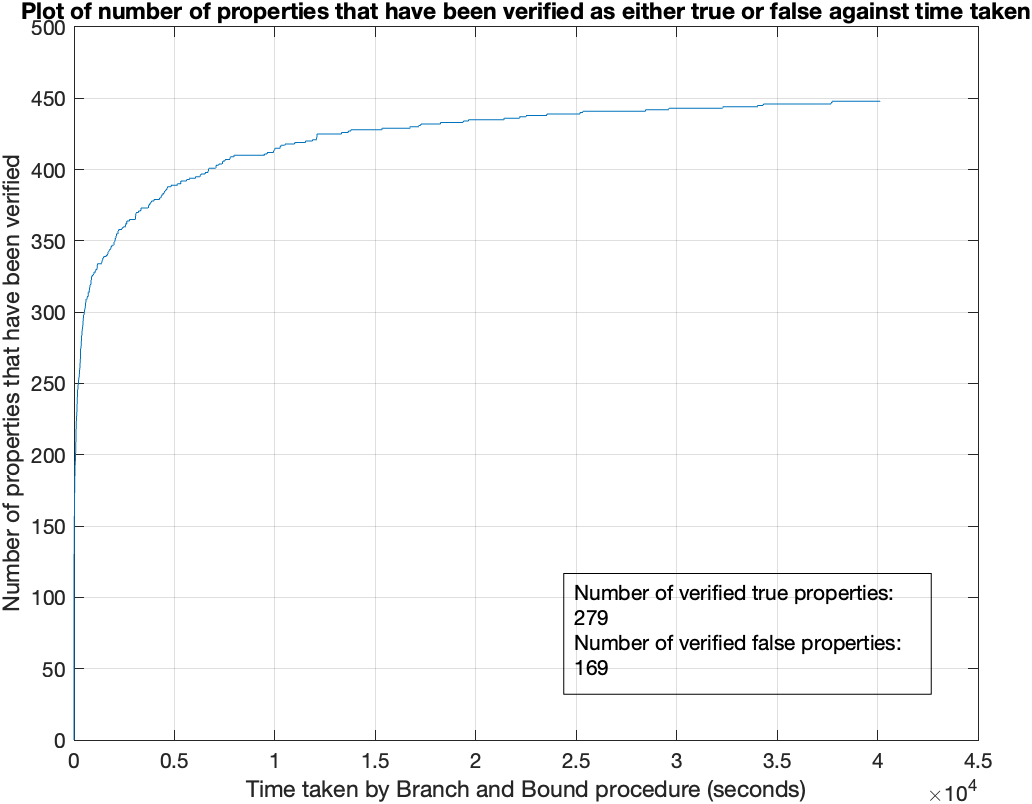
\includegraphics[width=7cm]{Task 3 (1 million) v2.png}
	\caption{Branch-and-bound}
	\label{fig:fig2}
\end{figure}

\section{Task 4: Projected Gradient Ascent for Lower Bounds}
\label{sec:Task 4}

Before coding the function, we have to look into how to to calculate the gradient of \emph{f}, which is the function that describes the neural network. By applying the chain rule, we get: 

\[
\pdv{f}{\textbf{x}} = {\left({\textbf{W}_5} {\pdv{ReLU(\hat{ \textbf{z}}_{4})}{\hat{ \textbf{z}}_{4}}} {\textbf{W}_4} {\pdv{ReLU(\hat{ \textbf{z}}_{3})}{\hat{ \textbf{z}}_{3}}} {\textbf{W}_3} {\pdv{ReLU(\hat{ \textbf{z}}_{2})}{\hat{ \textbf{z}}_{2}}} {\textbf{W}_2} {\pdv{ReLU(\hat{ \textbf{z}}_{1})}{\hat{ \textbf{z}}_{1}}} {\textbf{W}_1}\right)}^T
\]

Hence, the outputs $\hat{ \textbf{z}}_{i}$ are computed, and the derivative of the ReLU function is applied on each of them element-wise. The result will then have to be diagonalised to give ${\pdv{ReLU(\hat{ \textbf{z}}_{i})}{\hat{\textbf{z}}_{i}}}$ \cite{Stanford}. Note that there will be \emph{k} number of ${\pdv{ReLU(\hat{ \textbf{z}}_{i})}{\hat{\textbf{z}}_{i}}}$ for each value of \emph{i} if we have \emph{k} inputs. While we could loop through \emph{k}, it is better to construct a 3D array of \emph{k} number of ${\pdv{ReLU(\hat{ \textbf{z}}_{i})}{\hat{\textbf{z}}_{i}}}$ in the pages (MATLAB term for the third dimension). The MATLAB \emph{pagemtimes} function is then used to multiply all the terms together to obtain $\pdv{f}{\textbf{x}}$ for each of the \emph{k} inputs. This is akin to \textbf{array broadcasting} in NumPy.


\subsection{Average amount of time}

Similar to what was done in Task 1, the average amount of time is measured and calculated for each value of \emph{k} and then plotted against \emph{k} as seen in Figure 3a. Not surprisingly, the average amount of time increases as \emph{k} increases, and it appears to be a linear relationship.

\subsection{Average lower bound}

The average lower bound for each value of \emph{k} is obtained using a similar approach as that in Section \ref{sec:1.2}. In Figure 3b, there is a sharp increase from $\emph{k}=0$ to $\emph{k}=5$, before the plot levels off. Compared to Figure 1b, the levelling off starts at a lower value of \emph{k}, and the levelling off portion is flatter. This suggests that projected gradient ascent approaches the true maximum outputs of the neural network faster than the method in Task 1.

\subsection{Number of properties for which a counter-example is found}

This can be found using the approach in Section \ref{sec:1.3}. From Figure \ref{fig:fig3c}, it can be seen that for values of \emph{k} larger than 17, the plot does not change significantly. Hence, relatively small values of \emph{k} are enough to prove most but not all of the false properties. This is much better than the results in Task 1. As can be seen in Figure \ref{fig:fig1c}, the method in Task 1 is not close to proving all the false properties despite using a larger value of \emph{k}. Figure \ref{fig:fig3c} also suggests that a small minority of false properties are harder to prove than the rest. These harder-to-prove properties likely have a lot of local maxima that are non-positive, making it harder for the gradient ascent method to find a positive maxima. Due to the randomised nature of the inputs, whether the gradient ascent method can find any positive maxima for each of the inputs to a false property is down to luck. Of course, the larger the value of \emph{k}, the higher the chances of generating an input that is close enough to a positive maximum for the gradient ascent method to find it. Additionally, 171 of the false properties are proven multiple times for different values of \emph{k}. All 172 false properties are proven only once, at $\emph{k}=93$. This suggests that one property in particular is significantly harder to prove than the others, and that it was only proven false by luck as it was not proven false for $93<\emph{k}\leq100$ as can be seen in Figure \ref{fig:fig3c}. Indeed, re-running the code confirms that not all 172 false properties are guaranteed to be proven false. Hence, a value of \emph{k} larger than 100 will be required to increase the chances of finding all the false properties, which will be more computationally expensive. The step size and cutoff can also be tweaked to improve the performance of this method. That being said, projected gradient ascent is superior to the method in Task 1 and could be used to calculate lower bounds within branch-and-bound.

\begin{figure}[!htb]
  %\centering
  \hspace*{\fill}%
  \subfloat[Average time (over all properties) against \emph{k}]{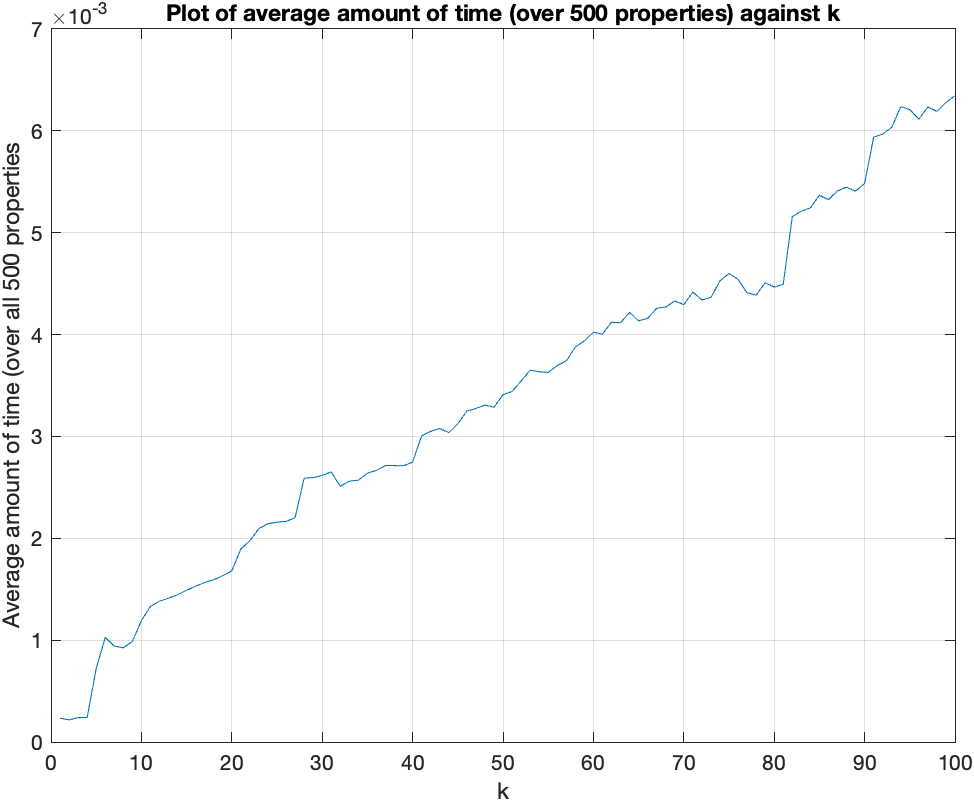
\includegraphics[width=7cm]{Task 4 average time (all).png}\label{fig:fig3a}}\hfill%
  %\hfill
  \subfloat[Average lower bound against \emph{k}]{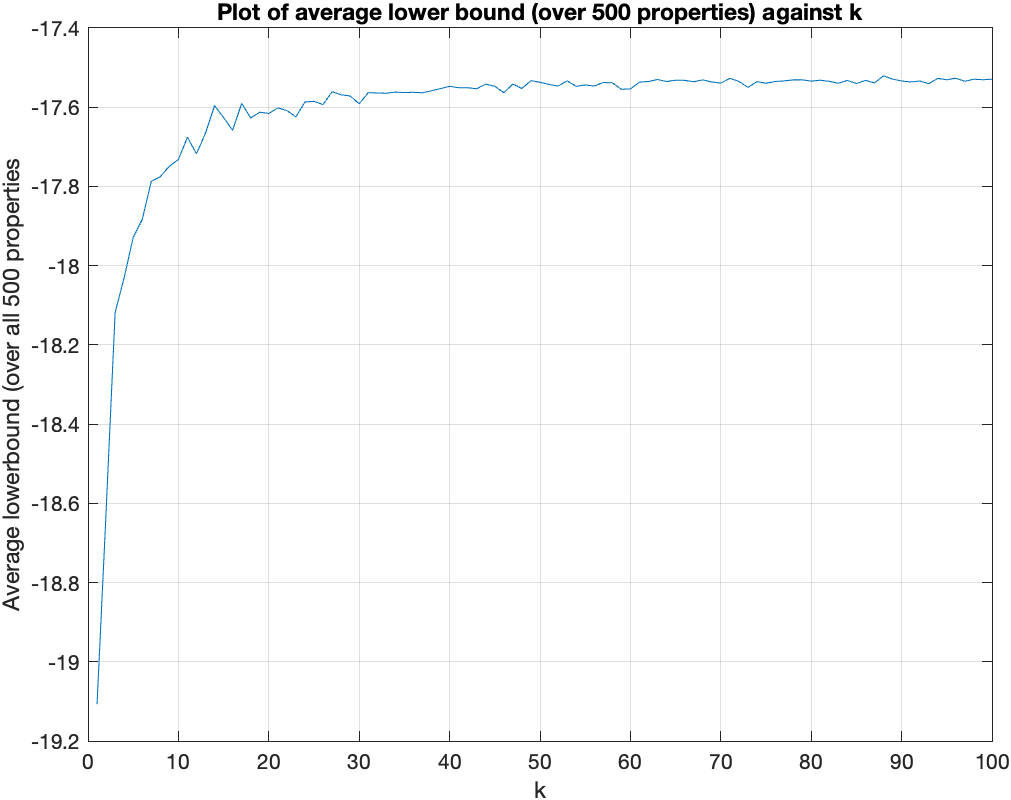
\includegraphics[width=7cm]{Task 4 average lower bound(all).png}\label{fig:fig3b}}\hfill%
  \hspace*{\fill}%
    %\hfill
  \hspace*{\fill}%
  \subfloat[Number of properties for which a counter-example is found against \emph{k}]{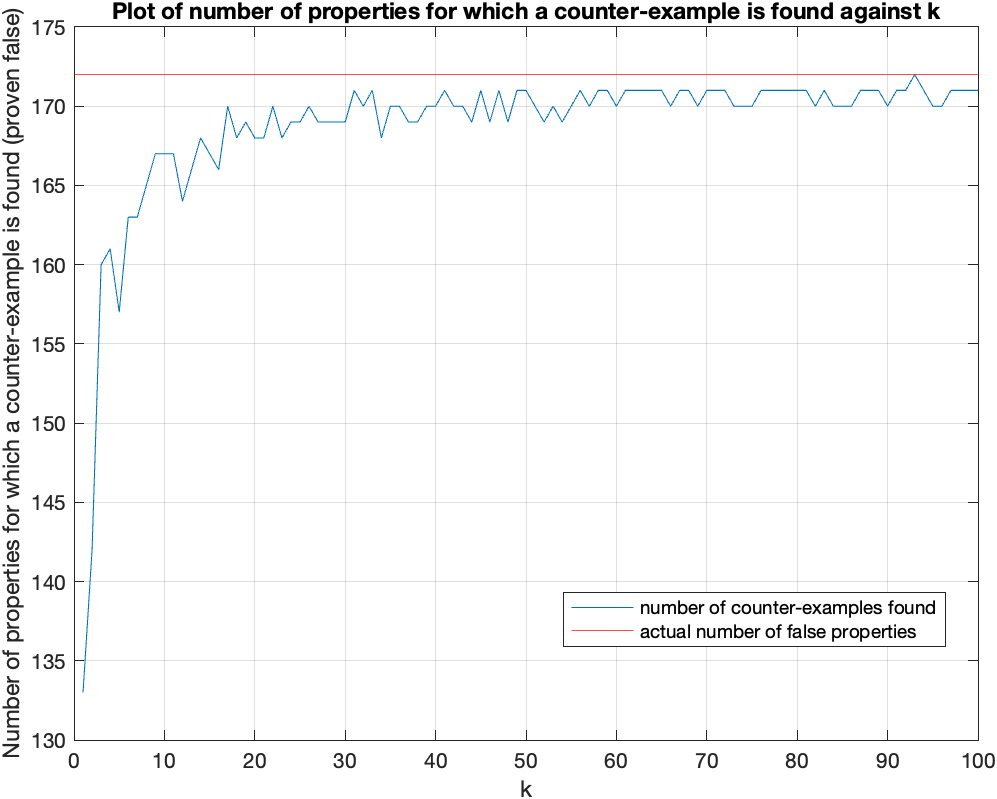
\includegraphics[width=7cm]{Task 4 counter examples (all proven).png}\label{fig:fig3c}}\hfill%
  \hspace*{\fill}%
  \caption{Projected Gradient Ascent (step size = 0.0005, cutoff = 0.00001)}
\end{figure}

\section{Task 5: Linear Programming Bound}
\label{sec:Task 5}

There are two ways to approach this: use linear programming on each layer of the network successively to obtain the bounds for $\hat{ \textbf{z}}_{k}$, $\textbf{z}_{k}$, and output y where $\emph{k}\in{\{1,2,3,4\}}$, or to use interval bound propagation to first obtain the bounds for $\hat{ \textbf{z}}_{k}$, $\textbf{z}_{k}$ and then these bounds in the linear programming applied on just the last layer. The latter approach is chosen for this task. Note that it does provide looser bounds but it is also less computationally expensive. 

We use \emph{linprog} to minimise 
\[
[\textbf{zeros}(1,261),\textbf{W}_{5}] [\textbf{x},\hat{ \textbf{z}}_{1},\textbf{z}_{1},\hat{ \textbf{z}}_{2},\textbf{z}_{2},\hat{ \textbf{z}}_{3},\textbf{z}_{3},\hat{ \textbf{z}}_{4},\textbf{z}_{4}]^T
\]
\[
-[\textbf{zeros}(1,261),\textbf{W}_{5}] [\textbf{x},\hat{ \textbf{z}}_{1},\textbf{z}_{1},\hat{ \textbf{z}}_{2},\textbf{z}_{2},\hat{ \textbf{z}}_{3},\textbf{z}_{3},\hat{ \textbf{z}}_{4},\textbf{z}_{4}]^T
\]

which is essentially minimising $y-b_5=\textbf{W}_{5}\textbf{z}_{4}$ and $-(y-b_5)=-\textbf{W}_{5}\textbf{z}_{4}$ respectively. Note that the variables that minimise $-(y-b_5)$ would maximise $y-b_5$. The inequality constraints matrices are assembled using the approximated linear inequality constraints:
\[
\textbf{z}_{k}(i) - C \hat{ \textbf{z}}_{k}(i) \leq -C {\hat{\textbf{z}}_k}^{min}(i), \text{where }C = \frac{{\hat{\textbf{z}}_k}^{max}(i)}{{\hat{\textbf{z}}_k}^{max}(i)-{\hat{\textbf{z}}_k}^{min}(i)}
\]
\[
\hat{ \textbf{z}}_{k}(i) - \textbf{z}_{k}(i) \leq 0,
\]
\[
\textbf{z}_{k}(i) \geq 0.
\]
Note that this third inequality constraint is already implied by the lower bounds calculated using interval bound propagation (since the lower bound of $\textbf{z}_{k}(i)$ must be non-negative), and hence can be omitted. However, these approximated constraints only apply if ${\hat{\textbf{z}}_k}^{min}(i)$ is negative and ${\hat{\textbf{z}}_k}^{max}(i)$ is positive. If both are negative, ${\textbf{z}_k}(i)$ is just zero. If both are positive, ${\textbf{z}_k}(i)$ is equal to ${\hat{\textbf{z}}_k}(i)$. Hence, we have to check the signs of every element of ${\hat{\textbf{z}}_k}^{min}(i)$, ${\hat{\textbf{z}}_k}^{max}(i)$ and modify the corresponding elements in the inequality constraints matrices by making them zero such that $0*{\hat{\textbf{z}}_k}(i) + 0*{\textbf{z}_k}(i) \leq 0$ if the approximated constraints do not hold. The equality matrices are also assembled accordingly such that $0*{\hat{\textbf{z}}_k}(i) + {\textbf{z}_k}(i) = 0$ for negative ${\hat{\textbf{z}}_k}^{min}(i)$ and ${\hat{\textbf{z}}_k}^{max}(i)$, and ${\hat{\textbf{z}}_k}(i) - {\textbf{z}_k}(i) = 0$ for positive ${\hat{\textbf{z}}_k}^{min}(i)$ and ${\hat{\textbf{z}}_k}^{max}(i)$. The $\hat{ \textbf{z}}_{k} - \textbf{W}_{k} \textbf{z}_{k-1} = 0$ (where $\textbf{z}_{0} = \textbf{x}$) constraints are also included in the equality matrices. All these constraints as well as the lower and upper bounds of the variables already calculated using interval bound propagation are then used within \emph{linprog} to minimise $y-b_5$ and $-(y-b_5)$. As mentioned before, this would give us the minimum and maximum value of $y-b_5$ respectively, which is essentially just the lower and upper bounds of y after adding $b_5$.

\subsection{Average value of the lower and upper bounds}
Similar to what was done in Section \ref{sec:221}, we obtain an average lower bound of -77.602404683211560 and an average upper bound of 14.819882426533335. This is a tighter bound than what was obtained in Task 2, especially the upper bound. Hence, we can expect this method to prove more properties.

\subsection{Number of properties proven}
Again, we re-use the code from Section \ref{sec:222} to show that 126 true properties and zero false properties are proven. While there is no difference in the number of proven false properties, there is a significant increase in number of proven true properties from 11 in Task 2 to 126. Hence, linear programming should be chosen over just interval bound propagation on its own when it comes to computing upper bounds.

\subsection{Incorporate linear programming bounds within Branch-and-bound}
\label{sec:5.3}

The code from Task 3 is modified to use linear programming to compute upper bounds instead of using interval bound propagation. However, it is not used to compute lower bounds given its poor performance at proving false properties. Instead, projected gradient descent from Task 4 is used. Figure \ref{fig:fig3c} shows that the plot levels off at around $\emph{k}=20$, so \emph{k} will be set to this value in this implementation of projected gradient ascent in order to balance between performance and computation cost. 

Running the modified code produces Figure \ref{fig:fig5}, which shows that all 500 properties are proven after $1.1607\times10^4$ seconds (roughly 3 hours). This algorithm only performed a maximum of 48966 partitions. This is vastly superior to the Task 3 algorithm, which was not able to prove all the properties even after 11 hours and a million partitions. It should also be noted that the majority of the properties were proven very early on, with a minority being significantly harder to prove. This is in line with what we observed in earlier tasks.



\begin{figure}[h]
	\centering
    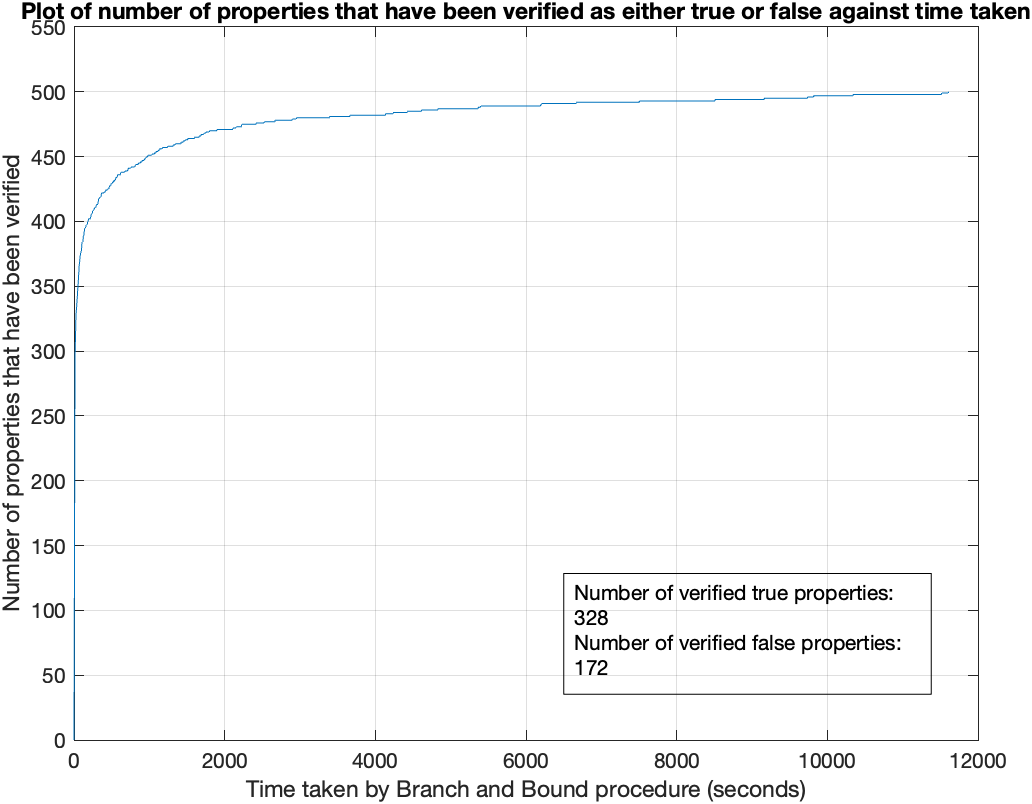
\includegraphics[width=8cm]{Task 5 bnb.png}
	\caption{Linear programming bound within branch-and-bound}
	\label{fig:fig5}
\end{figure}

\section{Test bench}
\label{sec:testbench}
We extract the information from \emph{groundtruth.txt} and put it in the vector \textbf{\emph{testbench}} such that the \emph{i}\textsuperscript{th} element is '1' if the \emph{i}\textsuperscript{th} property is true, and '-1' if false. For all the tasks in this report, \textbf{\emph{flag}} vectors with different notations had been used to count the number of proven properties. These vectors can be modified to follow the same notation as \textbf{\emph{testbench}} with '1' for proven true properties, '-1' for proven false properties, and '0' for unproven properties. Equating a modified \textbf{\emph{flag}} vector with \textbf{\emph{testbench}} will give a vector of logical '1's and '0's. Summing up all the elements in this vector should then give the total number of correctly proven properties. Since the number of proven properties for each of the tasks is already known, we check if the total number of correctly proven properties matches it. If so, the code for that particular task passes the test bench and can be taken to be correct. If there are any wrongly labelled properties (true property gets proven as false or vice versa), the two numbers would not match and the code would then have to be corrected. All the tasks have passed this test bench.

\section{Conclusion}
\label{sec:conclusion}
The method used in Section \ref{sec:5.3} is the only algorithm that proved all 500 properties within a reasonable amount of time. Hence, it seems that a branch-and-bound algorithm using both projected gradient ascent and linear programming would be best suited for network verification of this kind. However, it should be noted that not all combinations of the algorithms have been tested. The value of \emph{k} used in projected gradient ascent could also be tweaked in order to achieve better performance. Most importantly, all the algorithms in this report have only been tested on one dataset. More datatsets would be needed to test the robustness of the algorithms. To conclude, a good approach to a verification problem would be to use projected gradient ascent on its own to determine an optimal value of \emph{k}, and then use that value of \emph{k} within the Section \ref{sec:5.3} algorithm.
\\
\\
\begin{thebibliography}{9}

\bibitem{tictoc}
“Measure the Performance of Your Code,” Measure the Performance of Your Code - MATLAB \& Simulink - MathWorks United Kingdom. [Online]. Available: https://uk.mathworks.com/help/matlab/matlab\_prog/measure-performance-of-your-program.html. [Accessed: 08-Jan-2022]. 

\bibitem{hardware}
M. Knapp-Cordes and B. McKeeman, “Improvements to TIC and TOC functions for measuring absolute elapsed time performance in Matlab,” MATLAB \& Simulink, 2011. [Online]. Available: https://uk.mathworks.com/company/newsletters/articles/improvements-to-tic-and-toc-functions-for-measuring-absolute-elapsed-time-performance-in-matlab.html. [Accessed: 17-Dec-2021]. 

\bibitem{Trees}
E. A. Bender and S. G. Williamson, “Lists, Decisions and Graphs. With an Introduction to Probability,” 2010. [Online]. Available: https://cseweb.ucsd.edu/~gill/BWLectSite/Resources/LDGbookCOV.pdf. [Accessed: 19-Dec-2021]. 

\bibitem{Stanford}
K.  Clark, “Computing Neural Network Gradients.” [Online]. Available: 
\\
https://web.stanford.edu/class/cs224n/readings/gradient-notes.pdf. [Accessed: 30-Nov-2021]. 
\end{thebibliography}


\end{document}

